 \section{Parser Combinators for Path Querying}

Parser combinators provide a way to specify a language syntax in terms of functions and operations on them. 
A parser in this framework is usually a function which consumes a prefix of an input and returns either a parsing result or an error if the input is erroneous. 
Parsers can be composed by using a set of parser combinators to form more complex parsers. 
A parser combinators library provides with a set of basic combinators (such as sequential application or choice), and there can also be user-defined combinators. 
Most parser combinators libraries, including the Meerkat library, can only process the linear input --- strings or some kind of streams. 
We extend the Meerkat library to work on the graph input.


\subsection{The Set of Combinators}

First we introduce a small example graph which represent a map~\ref{fig:graph}.
There can be a road from one city to another, this relation is shown in graph as an edge with label $road\_to$.
Each city has name belongs to a country. 

{it may be useful to add types decalration for edge and vrt lables. Properties access (like .name, .country) will bw more evident}

And let we try to extract some information from this map.

\begin{figure}[h]
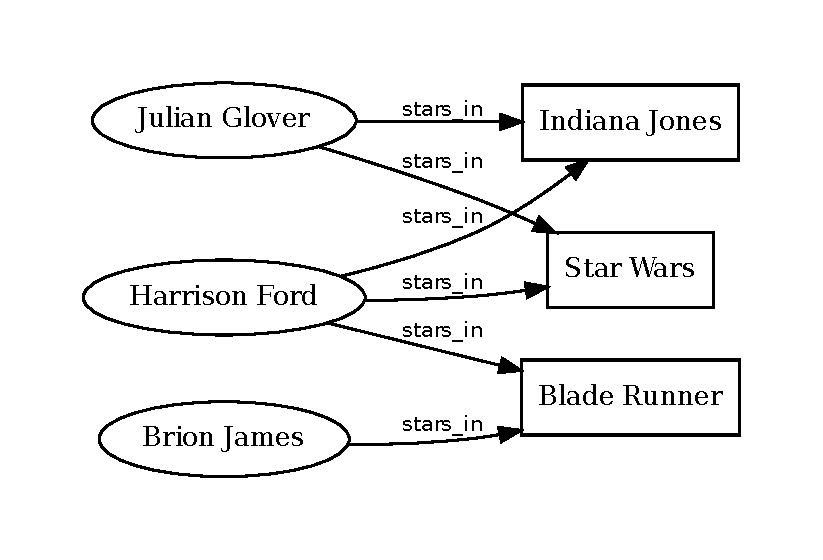
\includegraphics[width=0.45\textwidth]{graph}
\caption{Example Input Graph of Roads}
\label{fig:graph}
\end{figure}

First of all, for creating queries we need to work with edges and vertices.
There are two main functions for that:
\begin{itemize}
    \item \lstinline{V[L](predicate: L => Boolean)} combinator for working with vertices. Accepts a predicate and parses only vertices which satisfies that predicate
    \item \lstinline{E[N](predicate: N => Boolean)} combinator for working with edges. Accepts a predicate and parses only edges which satisfies that predicate  
\end{itemize}

\begin{figure}[h]
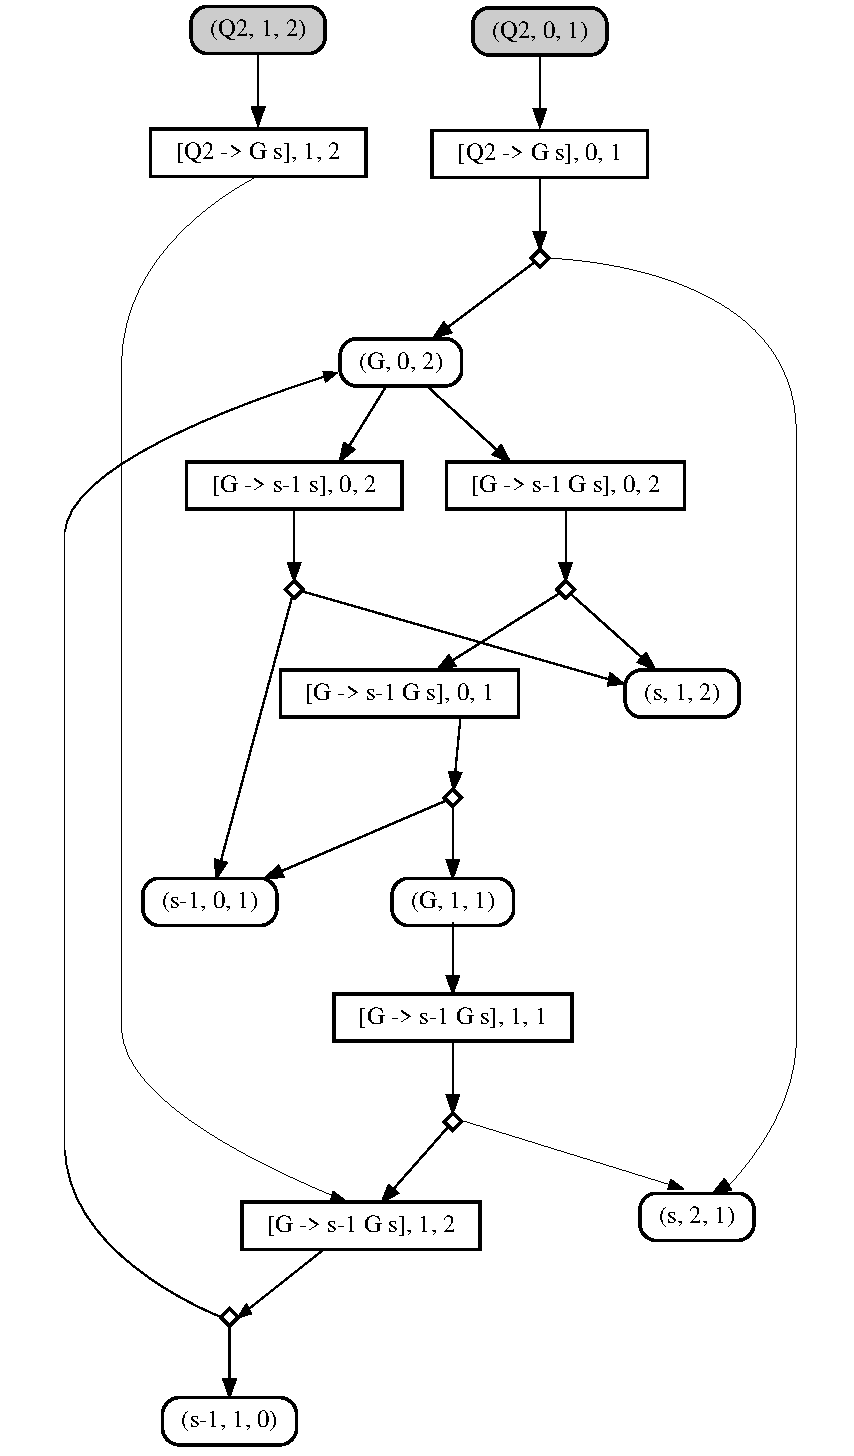
\includegraphics[scale=0.38]{sppf}
\caption{SPPF: result of applying actor/movie query to the graph~\ref{fig:graph}}
\label{fig:sppf}
\end{figure}

(Write sth about syn macro \\ I think it should be in section 2 in Meerkat description)


Suppose that we would like to select cities from our graph which belongs to some country. 
For that we use function \lstinline{V}: \lstinline{V[L]((e: Entity) => e.country = "County Name")}.
Here \lstinline{Entity} is a property container for graph entities: edges and vertices. 
Also, for the sake of simplicity, we will not explicitly specify \lstinline{Entity} type for predicates. 
Now let us build a query which gets all roads from city in $country0$ to city in $country$. 
For that we can use a sequentialital combinator \lstinline{~}. 
It allows to create queries which sequentialy applies two queries one after another. 
When we have subquery for retrieving a vertex with specific city, let's call it \lstinline{city(name: String)} and a subquery \lstinline{roadTo} for retrieving road edges. 
Let's finally build a query \lstinline{city("city0") ~ roadTo ~ city("city1")} which !!!!!.
The full query with subqueries is shown on fig. \ref{fig:simpleQuery}.

\begin{figure}[h]
\begin{lstlisting}
def city(country: String) =
  V(e.name == name)
val roadTo = E(_.value() == "road_to")
val ourPath = 
  city("country0") ~ roadTo ~ city("country1")
\end{lstlisting}
\caption{Path query}
\label{fig:simpleQuery}
\end{figure}



Now we would like to get all pair of cities which have a road between them. 
So we need to transform our query to use semantic actions which is described in \ref{sec:semanticActions} section. 
Now let us specify what we want from every our query. 
From the \lstinline{city} query we want only city name, so we need to map a result of basic vertex combinator. 
For that case we have a \lstinline{^} combinator we can write \lstinline{def city(name: String) = syn(V(e.value() == name) ^ (_.value))} to achive that. 
In \lstinline{ourPath} query we need first and second cities to be represented as a pair. 
For that we have a \lstinline{&} combinator which will map our sequence to a pair of strings.
The final representation is shown on \ref{fig:simpleQueryV2}. 
Now when we execute that query we will get a list which consists of all pairs of city's names which have a road between.

\begin{figure}[h]
\begin{lstlisting}
def city(country: String) =
  syn(V(e.country() == country) ^ (_.name))
val roadTo = E(_.value() == "road_to")
val ourPath = 
  syn(city("city0") ~ roadTo ~ city("city1") &
    {case c0 ~ c1 => (c1, c2)}
\end{lstlisting}
\caption{Path query}
\label{fig:simpleQueryV2}
\end{figure}


The whole set of basic combinators our library provides are presented in table~\ref{table:combinators}. 
It consists of two kind of combinators. The first kind creates new parsers from existing ones, meanwhile the second one allows mapping parsers result.
Parsers for matching strings are implicitly generated whenever a string is used within a query. 
The classical same generation query~\cite{FndDB} can be written using the library as presented in Fig.~\ref{fig:query1Meerkat}.



\begin{table}[h]
\centering
\begin{tabular}{l@{}|l}
\multicolumn{1}{c|}{Combinator} & \multicolumn{1}{|c}{Description} \\ \hline
{\lstinline!a ~ b!} & sequential parsing: {\lstinline!a!} then {\lstinline!b!}   \\
{\lstinline!a | b!} & choice: {\lstinline!a!} or {\lstinline!b!}         \\
{\lstinline!a ?!}   & optional parsing: {\lstinline!a!} or nothing   \\
{\lstinline!a *!}   & repetition of zero or more {\lstinline!a!} \\
{\lstinline!a +!}   & repetition of at least one {\lstinline!a!} \\
{\lstinline!a ^ f!} & apply {\lstinline!f!} function to {\lstinline!a!} if  {\lstinline!a!} is a token \\
{\lstinline!a ^^!}  & capture output of {\lstinline!a!} if {\lstinline!a!} is a token    \\
{\lstinline!a & f!} & apply {\lstinline!f!} function to {\lstinline!a!} if  {\lstinline!a!} is a parser \\
{\lstinline!a &&!}  & capture output of {\lstinline!a!} if {\lstinline!a!} is a parser    \\
\hline
\end{tabular}
\caption{Meerkat combinators}
\label{table:combinators}
\end{table}


\subsection{Generic interface for input}
Combinators is a way to describe a query. 
When we have a query we may want to execute that query on some graph considering it as an input for our query. 
The cool thing is that that input can be generalized to achive flexibility of all possible application of graph combinators and support a wide range of data sources. 
The idea is to present the input as two functions, one for working with edges and one for vertices. 
The first one would allow to get all edges outcoming from current vertex and also satisfies given predicate. 
The second one will allow to check if current vertex satisfies given predicate. That interface is presented on fig~.\ref{fig:input}.
We have implementation of that input for the next data sources: 

\begin{itemize}
    \item Neo4jInput --- input source for working with graph database Neo4J;
    \item GraphxInput --- input source for working with graph presented in memory using GraphX library;
    \item LinearInput --- input source for working with linear input data like strings.
\end{itemize}


\begin{figure}[h]
\begin{lstlisting}
trait Input[+L, +N] {
  def filterEdges(nodeId: Int, 
      predicate: L => Boolean): Seq[(L, Int)]
  def checkNode(nodeId: Int, 
      predicate: N => Boolean): Option[N]
}

\end{lstlisting}
\caption{Generalized input interface}
\label{fig:input}
\end{figure}


\subsection{Semantic Actions}
\label{sec:semanticActions}

Semantic actios !!!!!!
!!!!!!
!!!!!!!!!